\chapter{Background: Multiview Machine Learning: Concepts, Methods, and Limitations}\label{chap:background}
\minitoc

\section{Introduction to Machine Learning and Multiview Learning}

Machine learning automates data analysis, allowing models to learn patterns and make decisions. It is divided into three primary paradigms: supervised, unsupervised, and reinforcement learning. This thesis focuses on \textit{multiview machine learning}, a specialized domain dealing with data that contain multiple `views' or types of information. 

\subsection{The Focus of Multiview Learning}

Multiview learning is concerned with learning robust representations and identifying associations between different views. For example, in representing a person, the face image, voice, text, and gesture could be different views. These methods can be categorized as either unsupervised or self-supervised based on their goals and assumptions about the data-generating process.

\subsection{Machine Learning Vs Statistical Inference}
Machine learning aims to optimize out-of-sample performance, typically measured on a designated test set that the algorithm has never seen before. This emphasis on generalization to new, unseen data distinguishes it from statistical inference, where the primary concern is parameter estimation within a given sample, and hypothesis testing to infer population parameters.

\subsubsection{Training, Validation, and Test Sets}

In machine learning, a dataset is often divided into three subsets: the training set, the validation set, and the test set. The training set is used to train the model; the validation set is used to fine-tune model parameters and for hyperparameter tuning; and the test set serves to evaluate the model's generalization performance. 

\subsubsection{Cross-Validation}

Cross-validation is a technique used to assess the generalizability of the model by partitioning the original training dataset into a set of smaller train and test subsets. The model is trained on each combination of these subsets and validated on the remaining data. This provides multiple performance metrics, usually summarized by their mean and variance, offering a robust way to evaluate the model's out-of-sample performance.

\subsubsection{Holdout Method}

Sometimes a separate holdout set, distinct from the test set, is used for final model evaluation. This holdout set is not used during any part of the training or hyperparameter tuning process, serving as a final, unbiased performance metric.

\subsection{Types of Multiview Machine Learning}

Multiview machine learning encompasses a variety of techniques aimed at learning from data that have multiple sources or modalities, also known as 'views'. These techniques can be broadly classified into supervised, unsupervised, and self-supervised multiview learning, with some algorithms straddling the boundary between the two. 

\begin{figure}
    \centering
    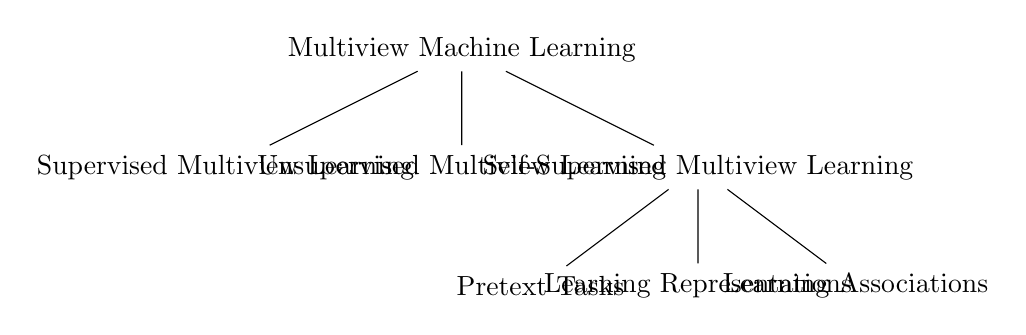
\begin{tikzpicture}[level distance=1.5cm,
    level 1/.style={sibling distance=3cm},
    level 2/.style={sibling distance=2cm}]
    
    \node {Multiview Machine Learning}
        child {node {Supervised Multiview Learning}}
        child {node {Unsupervised Multiview Learning}}
        child {node {Self-Supervised Multiview Learning}
            child {node {Pretext Tasks}}
            child {node {Learning Representations}}
            child {node {Learning Associations}}
        };
        
    \end{tikzpicture}
    \caption{Categories of Multiview Machine Learning}
    \label{fig:multiview_ml}
\end{figure}

\subsubsection{Supervised Multiview Learning}

In supervised multiview learning, one view serves as the input while the other view is treated as the target label. The algorithm learns to predict the target view based on the input view, leveraging the information from both to enhance the predictive performance. This approach is especially useful when each view contains complementary information that can improve the model's accuracy or robustness.

\subsubsection{Unsupervised Multiview Learning}

In unsupervised multiview learning, the primary focus is on capturing the inherent associations between different views without relying on explicit labels. For instance, Canonical Correlation Analysis (CCA) aims to find a common space where the correlation between different views is maximized. However, in this context, CCA does not inherently posit that these correlated views arise from a single latent source.

\subsubsection{Self-Supervised Multiview Learning}

Self-Supervised Learning (SSL) is a paradigm where the training signal is derived from the data itself, rather than relying on external labels. The cornerstone of SSL is the concept of a `pretext task,' a learning task created from the data that trains the model to capture useful features or representations. In the context of multiview machine learning, self-supervised learning operates under the assumption that different views are generated from a common latent variable. The pretext task, in this case, is to predict these latent variables from the given views. This not only enables the model to learn associations between views but also allows it to derive robust and informative representations for subsequent tasks like classification or regression.

\subsubsection{Blurred Boundaries}

While these categorizations provide a useful framework, it is important to note that the boundaries between unsupervised and self-supervised multiview learning are not always distinct. Algorithms like CCA can be interpreted differently based on context and specific datasets. In certain scenarios, CCA may function in an unsupervised manner by learning associations between

\section{Learning Representations: Definitions and Notation}

Suppose we have a sequence of vector-valued random variables $X^{(i)} \in \R^{D_i}$ for $i \in \{1, \dots, I \}$
We want to learn meaningful $K$-dimensional representations
\begin{equation}\label{eq:general-form-of-representations}
    Z\sps{i} = f\sps{i}( X\sps{i}; \theta\sps{i}).
\end{equation}
For convenience, define $D = \sum_{i=1}^I D_i$ and $\theta = \left(\theta\sps{i}\right)_{i=1}^I$.
Without loss of generality take $D_1 \geq D_2 \geq \cdots \geq D_I$.
We will consistently use the subscripts $i,j \in [I]$ for views;
$d \in [D_i]$ for dimensions of input variables;
and $l,k \in [K]$ for dimensions of representations - i.e. to subscript dimensions of $Z\sps{i}, f\sps{i}$.
Later on we will introduce total number of samples $N$.

In this report, we will typically refer to $u_k$ as \textbf{weights}, $Z_k = X_k u_k$ as \textbf{representations},
        \textbf{latent
dimensions}, or \textbf{scores} depending on the context. We will sometimes consider the
        matrix $U = \left(u_1, \dots, u_K\right) \in \R^{D \times K}$ of weights, and the
        matrix $Z = \left(Z_1, \dots, Z_K\right) \in \R^{N \times K}$ of representations. We will refer to $\mathbb{E
        }[X_k^\top X_k] u_k$ as loadings.

\subsection{Principal Components Analysis}

Principal Components Analysis (PCA)\cite{hotelling1933analysis} is a classical method in unsupervised machine learning for representation learning.
It is widely used for dimensionality reduction and feature extraction.
The primary goal of PCA is to transform the original high-dimensional data into a new coordinate system defined by orthogonal axes, capturing the most relevant aspects of the data.

In PCA, the representations are constrained to be linear transformations of the form:
\begin{equation}\label{eq:pca-linear-function-def}
    Z_k = X u_k,
\end{equation}
where $u_k$ are the orthonormal basis vectors:
\begin{equation}\label{eq:pca-orthonormality-constraint}
    u_k^\top u_l = \delta_{kl}.
\end{equation}

The primary goal of PCA is to maximize the variance of the projections \(Z_k\). Mathematically, this can be formulated
as:
\begin{align}
    u_{\text{opt}} &= \underset{u}{\text{argmax}} \left( u^\top X^\top Xu \right) \\
    \text{subject to:} \notag \\
    u^\top u &= 1 \notag
\end{align}

\paragraph{Optimization and Solution}
The Lagrangian for this problem is:
\begin{equation}
    f(u,\lambda) = u^\top X^\top Xu + \lambda(1 - u^\top u),
\end{equation}
where \(\lambda\) is the Lagrange multiplier. Differentiating the Lagrangian yields the first-order conditions:
\begin{align}
    X^\top X u &= \lambda u, \\
    u^\top u &= 1.
\end{align}

This transforms the problem into an eigenvalue equation for the covariance matrix \(X^\top X\), which can be efficiently solved using standard libraries such as scikit-learn\cite{pedregosa2011scikit}.

The first principal component corresponds to the eigenvector associated with the largest eigenvalue \(\lambda\). Subsequent components are ordered by their corresponding eigenvalues.

\textbf{Limitations: }However, when applying PCA to datasets such as high-dimensional neuroimaging and behavioral
data, PCA's main limitation arises: it only accounts for variance within a single dataset, potentially discarding features that are relevant for cross-modal analysis.

\subsection{Partial Least Squares}

Partial Least Squares (PLS)\cite{wold1975path} aims to maximize the shared covariance between two paired sets of data, referred to as `views". PLS can be seen as a generalization of PCA, where PCA becomes a special case when the two views are identical. The optimization problem for PLS can be formulated as:

\begin{align}
     u\sps{1}_{\text{opt}} &= \underset{u\sps{1}}{\mathrm{argmax}} \{ u\spstop{1} X\spstop{1} X\sps{2} u\sps{2} \} \\
     \text{subject to:} \notag \\
     u\spstop{1}u\sps{1} &= 1 \notag \\
     u\spstop{2}u\sps{2} &= 1 \notag
\end{align}

where \( X\sps{1} \in \mathbb{R}^{n \times p_1} \) and \( X\sps{2} \in \mathbb{R}^{n \times p_2} \), meaning we have two views with the same number of samples but potentially different number of features.

\subsubsection{Eigenvalue Problem}

The Lagrangian for this optimization problem can be formulated as:

\begin{equation}
f(u\sps{1}, \lambda) = u\spstop{1} X\spstop{1} X\sps{2} u\sps{2} + \lambda_1 (1 - u\spstop{1}u\sps{1}) + \lambda_2 (1 - u\spstop{2}u\sps{2})
\end{equation}

Upon deriving the first order conditions, we get:

\begin{align}
    X\spstop{2} X\sps{1} u\sps{1} &= \lambda_2 u\sps{2} \\
    X\spstop{1} X\sps{2} u\sps{2} &= \lambda_1 u\sps{1} \\
    u\spstop{1}u\sps{1} &= 1 \\
    u\spstop{2}u\sps{2} &= 1
\end{align}

By substituting the constraint conditions into these equations, we find that \( \lambda_1 = \lambda_2 = \lambda \) by symmetry. Further simplification yields:

\begin{align}
    X\spstop{2}X\sps{1} X\spstop{1} X\sps{2} u\sps{2} &= \lambda^2 u\sps{2} \\
    X\spstop{1}X\sps{2} X\spstop{2} X\sps{1} u\sps{1} &= \lambda^2 u\sps{1}
\end{align}

Thus, solving these equations will yield the \( u\sps{1} \) and \( u\sps{2} \) vectors as the eigenvectors of \( X\spstop{1} X\sps{2} X\spstop{2} X\sps{1} \) and \( X\spstop{2} X\sps{1} X\spstop{1} X\sps{2} \), respectively \cite{hoskuldsson1988pls}.

\textbf{Limitations: } The problem with applying PLS to neuroimaging and behavioural modalities is that PLS is not scale invariant and
is therefore biased towards the largest principal components in the data \cite{helmer2020stability}.
This is particularly problematic when there is a low signal to noise ratio since PLS may find directions in either dataset which correspond to the largest directions of noise in the other.
Additionally, PLS assumes that the structures contributing to variance in both datasets are linearly related, which
may not be the case in complex biological systems like the brain or in intricate behavioral patterns \cite{rosipal2005overview}.
The linearity assumption can sometimes be overly restrictive, failing to capture more complicated, nonlinear relationships between the data modalities.
Another issue is the lack of sparsity in the PLS solution.
Traditional PLS methods do not provide sparse weight vectors, which makes the interpretation of results challenging in high-dimensional settings such as neuroimaging where only a subset of features might be relevant \cite{leurgans1993canonical}.
There are sparse variants of PLS available, but these typically introduce additional complexity and may require fine-tuning of regularization parameters \cite{chun2010sparse}.
Furthermore, PLS can be sensitive to outliers, which are not uncommon in neuroimaging data due to motion artifacts or other sources of noise.
Since the method aims to maximize covariance, extreme values in one dataset can disproportionately affect the resulting latent variables \cite{wold1975path}.

\subsection{Canonical Correlation Analysis}\label{sec:cca}

In CCA, we aim to find the directions that maximize correlation, as opposed to maximizing covariance between two views of a dataset.
This nuance renders CCA invariant to feature scale. The optimization problem for CCA can be expressed as:

\begin{align}
     & u_{\text{opt}}=\underset{u}{\mathrm{argmax}}\{ u\spstop{1}X\spstop{1}X\sps{2}u\sps{2} \} \\
     & \text{subject to:} \notag \\
     & u\spstop{1}X\spstop{1}X\sps{1}u\sps{1}=1 \notag \\
     & u\spstop{2}X\spstop{2}X\sps{2}u\sps{2}=1 \notag
\end{align}

Although non-convex, numerous methods exist for solving the CCA problem, such as eigenvalue problems, generalized eigenvalue problems, block coordinate descent via alternating least squares regressions \cite{golub1995canonical,sun2008least} , and gradient descent \cite{via2007learning}.

\subsubsection{Eigenvalue Problem}

The first-order conditions derived in the same manner as the PLS case are:

\begin{align}\label{CCA:FOCs}
     & X\spstop{2}X\sps{1}u\sps{1}=\lambda\sps{2} X\spstop{2}X\sps{2}u\sps{2} \\
     & X\spstop{1}X\sps{2}u\sps{2}=\lambda\sps{1} X\spstop{1}X\sps{1}u\sps{1} \\
     & u\spstop{1}X\spstop{1}X\sps{1}u\sps{1}=1 \\
     & u\spstop{2}X\spstop{2}X\sps{2}u\sps{2}=1
\end{align}

Substituting the second two conditions into the first two, we get \(\lambda\sps{1}=\lambda\sps{2}=\lambda\). Then, recognizing \(X_i^{\top}X_i\) as the covariance matrix \(\Sigma_{ii}\) and \(X_i^{\top}X_j\) as the cross-covariance matrix \(\Sigma_{ij}\), we obtain another pair of eigenvalue problems:

\begin{align}
     & \Sigma_{11}^{-1}\Sigma_{12}\Sigma_{22}^{-1}\Sigma_{21}u\sps{1}=\lambda^2u\sps{1} \notag \\
     & \Sigma_{22}^{-1}\Sigma_{21}\Sigma_{11}^{-1}\Sigma_{12}u\sps{2}=\lambda^2u\sps{2} \notag
\end{align}

An alternative form of the CCA problem can be developed by reparameterizing \(u\sps{i*}=(X\spstop{i}X\sps{i})^{-\frac{1}{2}}u\sps{i}\). The optimization problem then becomes:

\begin{align}
     & u\sps{*}_{\text{opt}}=\underset{u\spstop{*}}{\mathrm{argmax}}\{ u\spstop{1*}(X\spstop{1}X\sps{1})^{-\frac{1}{2}}X\spstop{1}X\sps{2}(X\spstop{2}X\sps{2})^{-\frac{1}{2}}u\sps{2*} \} \\
     & \text{subject to:} \notag \\
     & u\spstop{1*}u\sps{1*}=1 \notag \\
     & u\spstop{2*}u\sps{1*}=1 \notag
\end{align}

This reparameterized form will later underpin Deep Canonical Correlation Analysis (DCCA).

This form also shows that PLS and CCA can be made equivalent by whitening the data matrices before constructing the covariance matrix. When the number of features exceeds the number of samples (\(p>n\)), CCA becomes degenerate because the within-view covariance matrices cannot be inverted—contrasting with PLS, which is always computable.

\subsubsection{Generalized Eigenvalue Problems}

We can also represent the system of equations in equation \ref{CCA:FOCs} as a matrix equation:

\begin{align}
    \begin{pmatrix}
        0                    & \Sigma_{12} \\
        \Sigma_{21} & 0
    \end{pmatrix}
    \begin{pmatrix}
        u\sps{1} \\
        u\sps{2}
    \end{pmatrix}
    =
    \lambda
    \begin{pmatrix}
        \Sigma_{11} & 0 \\
        0                    & \Sigma_{22}
    \end{pmatrix}
    \begin{pmatrix}
        u\sps{1} \\
        u\sps{2}
    \end{pmatrix}
\end{align}

Which is of the form $\mathbf{A v} = \lambda \mathbf{B v}$. CCA is therefore often referred to as a generalized eigenvalue problem for which there are a number of publicly available solvers.

\subsubsection{LDA as a Special Case of CCA}

Linear Discriminant Analysis (LDA) can be viewed as a special case of Canonical Correlation Analysis (CCA) where \(X^{(2)}\) is a one-hot encoded matrix representing the class labels.
This allows us to draw a connection between the unsupervised learning framework of CCA and the supervised framework of LDA, thus expanding the understanding of both algorithms.

\textbf{Intuition:} In LDA, the aim is to find a lower-dimensional subspace where the classes are maximally separated. This objective can be viewed through the lens of CCA, where the optimal directions \(u^{(1)}\) and \(u^{(2)}\) in the original and one-hot encoded spaces aim to maximize correlation. In the LDA context, \(u^{(1)}\) would maximize the separation between classes.

Mathematically, LDA is reduced to solving a generalized eigenvalue problem involving the between-class scatter matrix \(S_B\) and the within-class scatter matrix \(S_W\):

\[
    \hat{S_B} = \sum_{i=1}^{c} n_i (\mu_i - \mu)(\mu_i - \mu)\top
\]

\[
    \hat{S_W} = \sum_{i=1}^{c} \sum_{x \in X_i} (x - \mu_i)(x - \mu_i)\top
\]

\textbf{Connection to CCA:} When \(X^{(2)}\) is the one-hot encoded matrix of class labels, the CCA problem effectively tries to maximize the correlation between the feature vectors and their corresponding labels.
This turns out to be equivalent to maximizing the between-class variance in LDA while minimizing the within-class variance.
Thus, LDA can be thought of as a constrained form of CCA, tailored to classification tasks.

This perspective unifies the two algorithms and shows that the core objective—finding meaningful relationships or directions in the data—is shared between both CCA and LDA.

\textbf{Multi-view CCA} is a straightforward extension of CCA to the case of 3-or more datasets.
The optimization problem for MCCA can be stated as:
\begin{align}
     & u_{\text{opt}} = \underset{u}{\mathrm{argmax}} \sum_{i=1}^{m} \sum_{j=1, j \neq i}^{m} u\sps{i\top} X\sps{i\top} X\sps{j} u\sps{j} \\
     & \text{subject to:} \notag \\
     & \sum_{i=1}^{m} u\sps{i\top} X\sps{i\top} X\sps{i} u\sps{i} = 1 \notag
\end{align}

The generalized eigenvalue problem (GEP) can be written in matrix form as follows:

\begin{align}
    \mathbf{A} \mathbf{U} &= \lambda \mathbf{B} \mathbf{U} \\
    \mathbf{A} &= \begin{pmatrix}
        0 & \Sigma_{12} & \cdots & \Sigma_{1m} \\
        \Sigma_{21} & 0 & \cdots & \Sigma_{2m} \\
        \vdots & \vdots & \ddots & \vdots \\
        \Sigma_{m1} & \Sigma_{m2} & \cdots & 0
    \end{pmatrix}, \\
    \mathbf{B} &= \begin{pmatrix}
        \Sigma_{11} & 0 & \cdots & 0 \\
        0 & \Sigma_{22} & \cdots & 0 \\
        \vdots & \vdots & \ddots & \vdots \\
        0 & 0 & \cdots & \Sigma_{mm}
    \end{pmatrix}, \\
    \mathbf{U} &= \begin{pmatrix}
        u\sps{1} \\
        u\sps{2} \\
        \vdots \\
        u\sps{m}
    \end{pmatrix}.
\end{align}

\subsection{Sample Covariance and Population Covariance}
In the previous sections, the methods were described in terms of population covariance matrices such as \(\Sigma_{11}=\mathbb{E}[X\spstop{1} X\sps{1}]\), \(\Sigma_{22}=\mathbb{E}[X\spstop{2} X\sps{2}]\), and \(\Sigma_{12}=\mathbb{E}[X\spstop{1} X\sps{2}]\). These population covariances assume an underlying probability distribution from which the data are drawn.

\textbf{Sample Covariance:} In practical settings, we often do not have access to the entire population but only to a sample. Hence, we can utilize the Sample Average Approximation to estimate these covariances:

\[
    \hat{\Sigma}\sps{12} = \frac{1}{b-1} \bar{\mathbf{X}\sps{1}} \bar{\mathbf{X}\sps{2}}\top
\]

Here, \(b\) denotes the size of the minibatch, and \(\mathbf{X}\sps{1} \in \mathbb{R}^{p \times b}\) and \(\mathbf{X}\sps{2} \in \mathbb{R}^{q \times b}\) are the data matrices for the samples from \(X\sps{1}\) and \(X\sps{2}\), respectively. The bar over \(\mathbf{X}\sps{1}\) and \(\mathbf{X}\sps{2}\) signifies that these are centered versions of the matrices, i.e., the mean has been subtracted from each column.

\textbf{Practical Implications:} Using sample covariance matrices introduces some estimation error but allows us to apply the methods in real-world scenarios where population-level data are unattainable. Additionally, the use of minibatches provides a computationally efficient way to estimate these covariances in large-scale problems, at the cost of some additional statistical noise.

\textbf{Connection to Previous Methods:} The use of sample covariance matrices is directly applicable to algorithms like CCA and LDA. When replacing the population covariances \(\Sigma\sps{ij}\) with sample estimates, the optimization problems remain structurally similar but are solved using the sample data.

This dual perspective—considering both population and sample covariance matrices—enables a more robust and flexible approach to the methods discussed, bridging the gap between theoretical analysis and practical application.

\subsection{Multiple Effects, Orthogonality, and Deflation}\label{subsec:orthogonality}

Understanding multiple correlated or covarying effects is fundamental in multivariate data analysis methods such as Principal Component Analysis (PCA), Partial Least Squares (PLS), and Canonical Correlation Analysis (CCA). Although these methods generally aim to find a single maximal correlation or covariance (referred to as the top-1 problem), they are capable of identifying more than one orthogonal effect, a scenario often termed the top-$k$ problem, where $k$ denotes the number of orthogonal effects desired.

\subsection{Challenges in Identifying Multiple Components}

Identifying multiple components using iterative methods introduces specific challenges.
Firstly, to discover subsequent effects that are orthogonal to the maximally correlated or covarying one, a deflation step is commonly applied.
This is essential because the second component is conditional on the first in deflation models, meaning that interpreting the second component as an independent form of variation becomes untenable if the wrong first component is identified.

\subsection{Deflation Methods for Orthogonality}

Two prevalent deflation methods, Hotelling's Deflation and Projection Deflation, serve to ensure the orthogonality of the components.

\textbf{Hotelling's method}  is mainly used for methods based on the power method for the Singular Value
Decomposition (SVD).

\begin{align}
     & d = \mathbf{w^{\top}_1X^{\top}_1X_2w_2}                                            \\
     & \mathbf{\Sigma^{(i+1)}_{12}}= \mathbf{\Sigma^{(i)}_{12}} - d\mathbf{w_1w^{\top}_2}
\end{align}

\textbf{Projection Deflation} is common in algorithms like Wold's NIPALS and ensures that the projection vectors
themselves are orthogonal. These methods work by systematically reducing the data dimensions, so that each new component is orthogonal to the ones found before it. However, these methods come with their own limitations and are sensitive to the condition of the original problem, including issues related to regularization.

\begin{align}
     & P(\mathbf{X})= \frac{\mathbf{Xw}}{\|\mathbf{Xw}\|}\mathbf{w^{\top}X^{\top}X}
\end{align}

\begin{align}
     & P^\perp(\mathbf{X})= \mathbf{X} - \frac{\mathbf{Xw}}{\|\mathbf{Xw}\|}\mathbf{w^{\top}X^{\top}X} = (I - \frac{\mathbf{Xw}}{\|\mathbf{Xw}\|}\mathbf{w^{\top}X^{\top})X}
\end{align}

\subsection{Non-Uniqueness of Components}

Another critical consideration is the non-uniqueness of the identified components.
The eigenvectors of covariance matrices in these methods are only defined up to a sign, or up to an orthogonal transformation when eigenvalues are repeated. This lack of uniqueness can lead to inconsistencies, especially when comparing solutions across different samples or data folds.

\subsection{Thesis Perspective}

Given these complexities, this thesis adopts a subspace perspective, focusing on either the top-1 or top-$k$ solutions, considering these as the most reliable and interpretable representations of the data's underlying structure.
This approach aims to mitigate the limitations of deflation methods and the non-uniqueness of solutions, providing a more robust framework for multivariate data analysis.

\section{Open challenges in CCA}

\subsection{Efficient Algorithms for High-Dimensional Data}

The challenges of high-dimensional data often manifest when solving Generalized Eigenvalue Problems (GEPs) for Canonical Correlation Analysis (CCA). The computational burden of solving these problems becomes daunting as the number of features grows. To combat this issue, various efficient algorithms have been developed to reduce the complexity. In this section, we will explore some of these strategies.

\subsubsection{Challenges in Solving Generalized Eigenvalue Problems}

The GEP is often represented as \( Ax = \lambda Bx \), where \( A \)and \( B \)are matrices whose dimensions depend on the method in use.
For instance, in PCA, \( A \) and \( B \)are \( p \times p \); in PLS and CCA, they are \( (p+q) \times (p+q) \).

% Table summarizing the definitions of A and B for various methods
\begin{table}[h]
    \centering
    \begin{tabular}{|c|c|c|c|c|}
        \hline
        Method & \( A \)&\( B \)&\( x \)& Dimensions\\
        \hline
        PCA& \( \Sigma_{11} \)&\( I \)&\( u\sps{1} \)&\( p \times p \) \\
        \hline
        LDA& \( S_B \)&\( S_W \)&\( u\sps{1} \)&\( p \times p \) \\
        \hline
        CCA& \( \begin{pmatrix} \Sigma_{11} & \Sigma_{12} \\ \Sigma_{21} & \Sigma_{22} \end{pmatrix} \)&\( \begin{pmatrix} \Sigma_{11} & 0 \\ 0 & \Sigma_{22} \end{pmatrix} \)&\( \begin{pmatrix} u\sps{1} \\ u\sps{2} \end{pmatrix} \)&\( (p+q) \times (p+q) \) \\
        \hline
        PLS& \( \begin{pmatrix} 0 & \Sigma_{12} \\ \Sigma_{21} & 0 \end{pmatrix} \)&\( I \)&\( \begin{pmatrix} u\sps{1} \\ u\sps{2} \end{pmatrix} \)&\( (p+q) \times (p+q) \) \\
        \hline
    \end{tabular}
    \caption{Definitions and dimensions of \( A \)and \( B \)for different subspace learning methods.}
    \label{tab:subspace}
\end{table}

To solve the GEP, one common technique is to transform it into a standard eigenvalue problem\( B^{-\frac{1}{2}} A B^{-\frac{1}{2}} y = \lambda y \), followed by eigendecomposition.
However, this approach has computational complexity \(O(n^3)\)and may suffer from numerical instability.

\subsubsection{PCA-CCA}

One way to reduce the complexity of solving GEPs is to use the PCA-CCA method, which first applies PCA to the data
and then solves the GEP in the reduced space. The primary advantage of using PCA-CCA is computational efficiency, especially for high-dimensional data.
The overall complexity of PCA-CCA is\(O(p^2K + p^3)\), where \( K \)is the number of reduced components.
This method is particularly beneficial when \( p \)is large.

\subsubsection{KCCA}

Kernel Canonical Correlation Analysis (KCCA) extends CCA to capture nonlinear relationships. The optimization problem for KCCA is:

\begin{align}
    & \alpha_{\text{opt}}=\underset{\alpha_{\text{opt}}}{\mathrm{argmax}}\{ \alpha_1^{\top}K\spstop{1}K\sps{2}\alpha_2  \}\\
    & \text{subject to:} \notag\\
    & \alpha_1^{\top}K\spstop{1}K\sps{1}\alpha_1=1 \notag\\
    & \alpha_2^{\top}K\spstop{2}K\sps{2}\alpha_2=1 \notag
\end{align}


KCCA is computationally efficient for high-dimensional data (\(p>n\)) because its complexity scales with the number of samples\(n\), not the number of features\(p\).
However, it requires access to all training data at test time, raising efficiency concerns.

\subsection{Non-linear CCA}

\subsubsection{Kernel CCA}

Kernel CCA (KCCA) is a non-linear extension of CCA that uses the kernel trick to find non-linear relationships between variables.

\subsubsection{Deep CCA}

Deep CCA (DCCA) is a non-linear extension of CCA that uses deep neural networks to find non-linear relationships between variables.

\section{Multiview Learning in Neuroimaging}

There have been a number of applications of CCA and related methods to multiview problems in neuroimaging.
Using resting state fMRI data, modes of correlation have been found that relate to differences in sex and age relating to drug and alcohol abuse, depression and self harm \cite{mihalik2019brain}.
A similar mode relating to `positive-negative' wellbeing has been found across studies \cite{smith2015positive}suggesting that mental wellbeing has a relationship (though not necessarily causally) with functional connectivity between networks in the brain.
Later in this dissertation we will replicate and build on the findings from this paper by using regularised and non-linear CCA methods.

CCA has also been used as a preprocessing step in order to identify groups of subjects in the latent variable space.
In particular, CCA and clustering have been used to identify depression using fMRI data\cite{dinga2019evaluating} \cite{drysdale2017resting}.
CCA has also been used in the manner we described to denoise two views of a dataset such as separate measures of neuroimaging data \cite{zhuang2020technical} to remove artefacts.
Deep CCA has recently been used to extract features for the diagnosis of schizophrenia\cite{qi2016deep}.





